% Fencing an agent in: layers, each with an honest limit.
% ---------------------------------------------------------------------------
% style.tex --- shared preamble for every figure in book/figures/tikz/
%
% One style for all figures: Latin Modern, thin black lines, a light grey
% fill, and one accent colour used only to mark what is untrusted or wrong.
% Build with scripts/build_figures.sh; see book/figures/README.md.
% ---------------------------------------------------------------------------
\documentclass[tikz,border=6pt]{standalone}
\usepackage[T1]{fontenc}
\usepackage{lmodern}
\usetikzlibrary{arrows.meta,positioning,shapes.geometric,calc,fit,backgrounds}

\hyphenpenalty=10000   % short lines in boxes: ragged, never hyphenated

\definecolor{lightgrey}{gray}{0.92}
\definecolor{accent}{HTML}{9B2D20}

\tikzset{
  every picture/.style={
    line width=0.6pt,
    font=\small,
    >={Stealth[length=5pt,width=4pt]},
    node distance=14pt and 24pt,
  },
  % shapes
  box/.style={draw, rectangle, inner xsep=8pt, inner ysep=5pt,
              minimum height=22pt, align=center},
  grey/.style={box, fill=lightgrey},
  rounded/.style={box, rounded corners=9pt},
  decision/.style={draw, diamond, aspect=2.4, inner sep=1.5pt, align=center},
  group/.style={draw, dashed, rounded corners=5pt, inner sep=7pt},
  % text
  tag/.style={font=\footnotesize, align=center, inner sep=2pt},
  note/.style={font=\footnotesize\itshape, align=center, inner sep=2pt},
  code/.style={font=\small\ttfamily},
  codetag/.style={font=\footnotesize\ttfamily, align=center, inner sep=2pt},
  title/.style={font=\small\scshape, align=center, inner sep=2pt},
  % lines
  arrow/.style={->},
  back/.style={->, dashed},
  thin/.style={line width=0.4pt, gray},
  % the one accent, for what is untrusted, wrong or missing
  bad/.style={accent},
  badbox/.style={box, draw=accent, text=accent},
}

\begin{document}
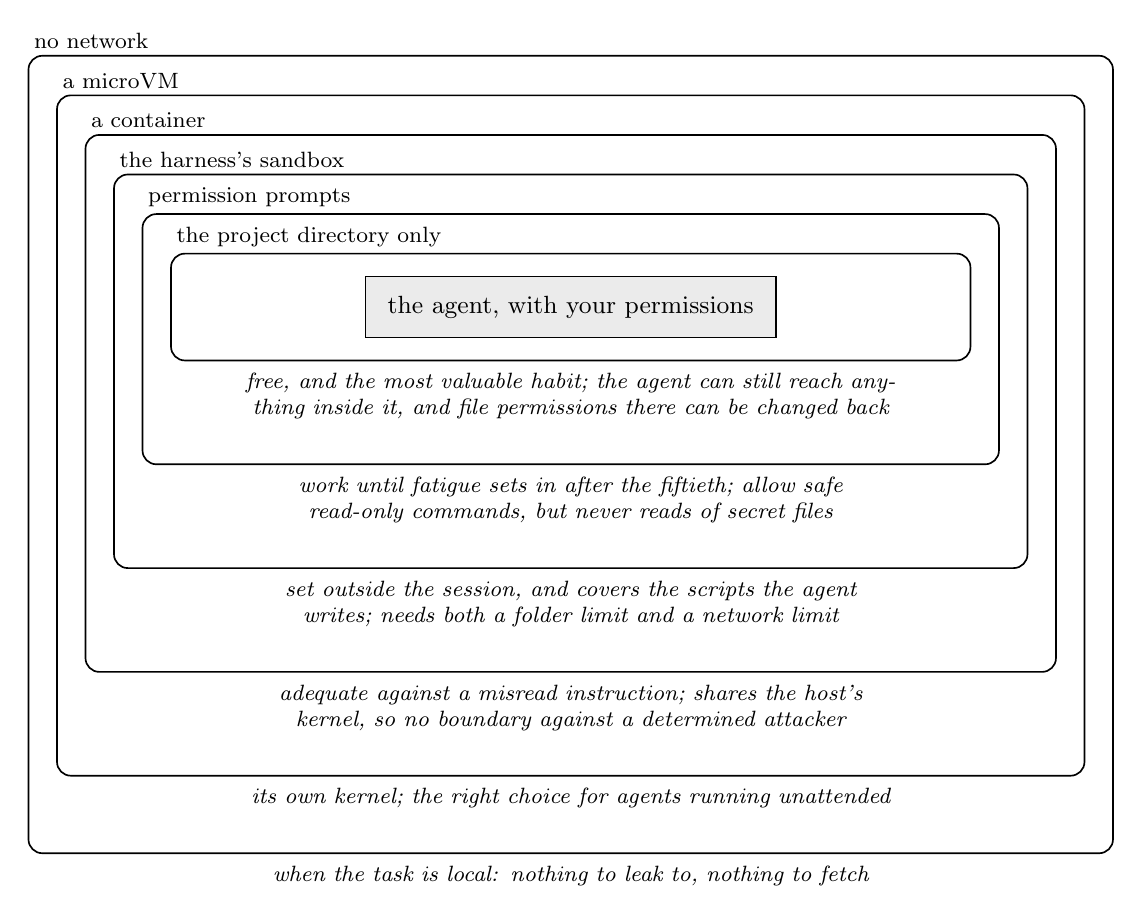
\begin{tikzpicture}[w/.style={note, text width=280pt}]
  \node[grey] (agent) at (0,0) {the agent, with your permissions};
  \node[group, solid, fit=(agent), inner xsep=70pt, inner ysep=8pt] (dir) {};
  \node[tag, anchor=south west] at (dir.north west) {the project directory only};
  \node[w, below=2pt of dir] (n1) {free, and the most valuable habit; the agent can still reach anything inside it, and file permissions there can be changed back};
  \node[group, solid, fit=(dir) (n1), inner xsep=10pt, inner ysep=14pt] (prompts) {};
  \node[tag, anchor=south west] at (prompts.north west) {permission prompts};
  \node[w, below=2pt of prompts] (n2) {work until fatigue sets in after the fiftieth; allow safe read-only commands, but never reads of secret files};
  \node[group, solid, fit=(prompts) (n2), inner xsep=10pt, inner ysep=14pt] (sand) {};
  \node[tag, anchor=south west] at (sand.north west) {the harness's sandbox};
  \node[w, below=2pt of sand] (n3) {set outside the session, and covers the scripts the agent writes; needs both a folder limit and a network limit};
  \node[group, solid, fit=(sand) (n3), inner xsep=10pt, inner ysep=14pt] (cont) {};
  \node[tag, anchor=south west] at (cont.north west) {a container};
  \node[w, below=2pt of cont] (n4) {adequate against a misread instruction; shares the host's kernel, so no boundary against a determined attacker};
  \node[group, solid, fit=(cont) (n4), inner xsep=10pt, inner ysep=14pt] (vm) {};
  \node[tag, anchor=south west] at (vm.north west) {a microVM};
  \node[w, below=2pt of vm] (n5) {its own kernel; the right choice for agents running unattended};
  \node[group, solid, fit=(vm) (n5), inner xsep=10pt, inner ysep=14pt] (net) {};
  \node[tag, anchor=south west] at (net.north west) {no network};
  \node[w, below=2pt of net] (n6) {when the task is local: nothing to leak to, nothing to fetch};
\end{tikzpicture}
\end{document}
